\documentclass[12pt,english]{article}
\usepackage{mathptmx}

\usepackage{color}
\usepackage[dvipsnames]{xcolor}
\definecolor{darkblue}{RGB}{0.,0.,139.}

\usepackage[top=1in, bottom=1in, left=1in, right=1in]{geometry}

\usepackage{amsmath}
\usepackage{amstext}
\usepackage{amssymb}
\usepackage{setspace}
\usepackage{lipsum}
\usepackage{longtable}
\usepackage{caption}
\usepackage{subcaption}
\usepackage{multirow}
\usepackage{float}
\usepackage{geometry}
\usepackage{tabularx}
\usepackage{rotating}
\usepackage[authoryear]{natbib}
\usepackage{url}
\usepackage{booktabs}
\usepackage[flushleft]{threeparttable}
\usepackage{graphicx}
\usepackage{pdflscape}
\usepackage[unicode=true,pdfusetitle,
 bookmarks=true,bookmarksnumbered=false,bookmarksopen=false,
 breaklinks=true,pdfborder={0 0 0},backref=false,
 colorlinks,citecolor=black,filecolor=black,
 linkcolor=black,urlcolor=black]
 {hyperref}
\usepackage[all]{hypcap} % Links point to top of image, builds on hyperref
\usepackage{breakurl}    % Allows urls to wrap, including hyperref

\linespread{2}

\begin{document}

\begin{singlespace}
\title{Implications of Review Scores on Video Game Sales}
\end{singlespace}

\author{Hayden Truong/ Thomas Joyce/ Jerry Hong}
% \date{\today}
\date{May 5th, 2024}


\maketitle

\begin{abstract}
\begin{singlespace}
Do reviews from official sources or consumers effect the sales of video games? In the world of 
entertainment products, where information asymmetry is abundant reliable signals of product 
quality are likely to be highly valued. However, in a world in which people can go on massive 
review bombing sprees out of protest, and official sources are known to have deals with large 
companies to rate games favorably, the role of reviews as a proper informational source of 
quality comes into question. In order to empirically estimate and separate the effects of these two 
signals, we analyze a sample of about 16,500 video games and their sales figures between 1980 
and 2016 and regress these figures on the official and consumer scores they received, using a 
number of regression methods to establish a clear picture of what effect is present. Upon 
conducting this analysis, we find that not only does simply having a critic score and user scores 
provide a distinct boost to sales, but having positive reviews in both of these areas can greatly 
improve the sales of the game, with critic scores appearing to have the most drastic effect. From 
these findings, this implies for businesses that the aspect of receiving reviews is extremely 
important for the returns on a gaming project. To this end, hiring professional sources to review 
their products is a particularly useful investment to ensure a game sells well. On another note, the 
aspect of critic reviews holding a much stronger effect than their consumer counterparts appears 
to imply a notion of a influence effect on other sources of information which is consistent with 
previous literature on the topic. 
\end{singlespace}

\end{abstract}
\vfill{}


\pagebreak{}
\tableofcontents
\pagebreak

\section{Introduction}\label{sec:intro}
Of the main industries in the entertainment sector, the gaming industry is perhaps one of the most 
profitable worldwide outperforming the movie, TV, and even music market by a large margin. In 
all of these industries, information plays a distinct role in the popularity of certain products, with 
a large amount of funding in these industries going towards advertising in order to convey 
positive information about a product to consumers. To this end, one might assume that one of the 
biggest drivers of the gaming industries success would be its ability to convey this important 
information component to its consumers well to ensure that audiences that will enjoy their 
product get to know about it. However, in one of the main components of conveying this 
information in the gaining industry, reviews, faces a large scale problem. While perhaps one of 
the largest sources of information on a gaming product, with thousands of consumer reviews, 
plenty of official sources for scores, and a multitude of channels dedicated to properly examining 
a product, one runs into the issue of trying to discern what information is useful in this large 
pool. In particular, it’s been known that many review based channels and sources strike deals 
with gaming companies to provide positive reviews for their games, and similarly, user reviews 
have been known to be used for protesting through review bombs, and many reviews are simply 
posted as jokes by a community. This particular nature of gaming reviews thus leaves their 
ability to convey information to the public properly in question and whether they actually have 
any particular effect on the sales of a game. To this end we hope to investigate this question on 
how reviews effect the sales of a game and to what degree throughout this paper while 
accommodating for various variables such as the year and console which also have a distinct 
effect on the sales of the game. Through this, we should be able to not only investment in 
reviews as a strategy for game companies, but also whether reviews are seen as a credible source 
of information in the current industry sphere.

\section{Literature Review}\label{sec:litreview}
In previous literature established by Arias (2019) \cite{canto2019effect} it has been shown that reviews do not appear to effect the shares of publisher companies, rather these shares move mostly with the market. This generally implies that reviews regardless of being from professional sources or by consumers have little effect on game sales, as if this was true, one would expect that a influx of 
negative reviews would effect a companies shares as they would be making little revenue. 
However, when examining the work of Kaimann (2015)\cite{cox2015reviews} reviews have a significantly positive effect on the sales of games. In particular, this work finds that reviews from official sources have a significant positive effect on sales that even outweighs those of consumers, as these official reviews create a unique influence effect on how the game in perceived. The logic here makes 
sense, as with the general information asymmetry around games positive indicators of quality 
should have a positive influence. Yet despite this, when we look at the work of Adigüzel (2021) \cite{adiguzel2021youtube}, 
we find another contradiction, as he finds that consumer reviews have the highest positive impact 
on sales and YouTube reviews posted by an influencer had only a similar effect as those put of by 
companies. If an influence effect was present in the gaming industry, one would expect that 
reviews posted by influencers should have a notable effect on other reviews yet despite this not 
such effect appears to occur. These three main contradictory findings seen in the literature may 
by due to the time period they are working with. In particular, Kaimann (2015) uses a set from 
2004 to 2010 while Adigüzel (2021) uses a set from 2010-2019. This is important, as from 2004 
to 2019, the perception of official reviews has diminished greatly, with many consumers 
understanding that these official sources can be bought of for a good review, which in turn 
shifted the perception of reliability to consumer reviews. Similarly, in 2004 the availability of 
information is much sparser to the later 2010’s which in general would shift the focus from 
official sources. By examining a broader dataset from around 2000 to 2016, we hope to 
consolidate these observed effects in previous literature to provide a more holistic examination of 
the effects of the various review types over time on game sales as a contribution to provide a 
distinct foundation for further research. 

\section{Data}\label{sec:data}
The primary data source for this research is courtesy of Kaggle by user \textit{Sid\_Twr}. The data set contains roughly 16,500 observations for games sold between 1980 to 2016. The data is motivated by Gregory Smith's data scraping from VGChartz Video Games Sales. This extends to incorporating critic and user reviews from Metacritic. The features contain the title of the game, the year it was released, the gaming platform it was launched on, the developer and publishers of the game, and total sales divided into four regions (North America (NA), European Union (EU), Japan (JP), and Other). The most important variable - global sales - which takes the cumulative number of sales among the four sub-regions, is the main variable we will be using in our regressions. Further details can be found in the documentation of the data. We begin some basic data analysis to understand the sales data. Below are a few graphs depicting sales revenue and volumes in general. Comprehensive summary statistics can be found in Table \ref{tab:descriptive-vg}.

We notice that historically the video game industry was growing exponentially in sales revenue until it experienced a decline in the last decade. Region-wise, North America and Europe remain the most profitable markets for gaming companies as together they account for about 50 percent of world wide demand. 

\begin{figure}[ht]
\centering
\begin{subfigure}{0.49\linewidth}
    \centering
    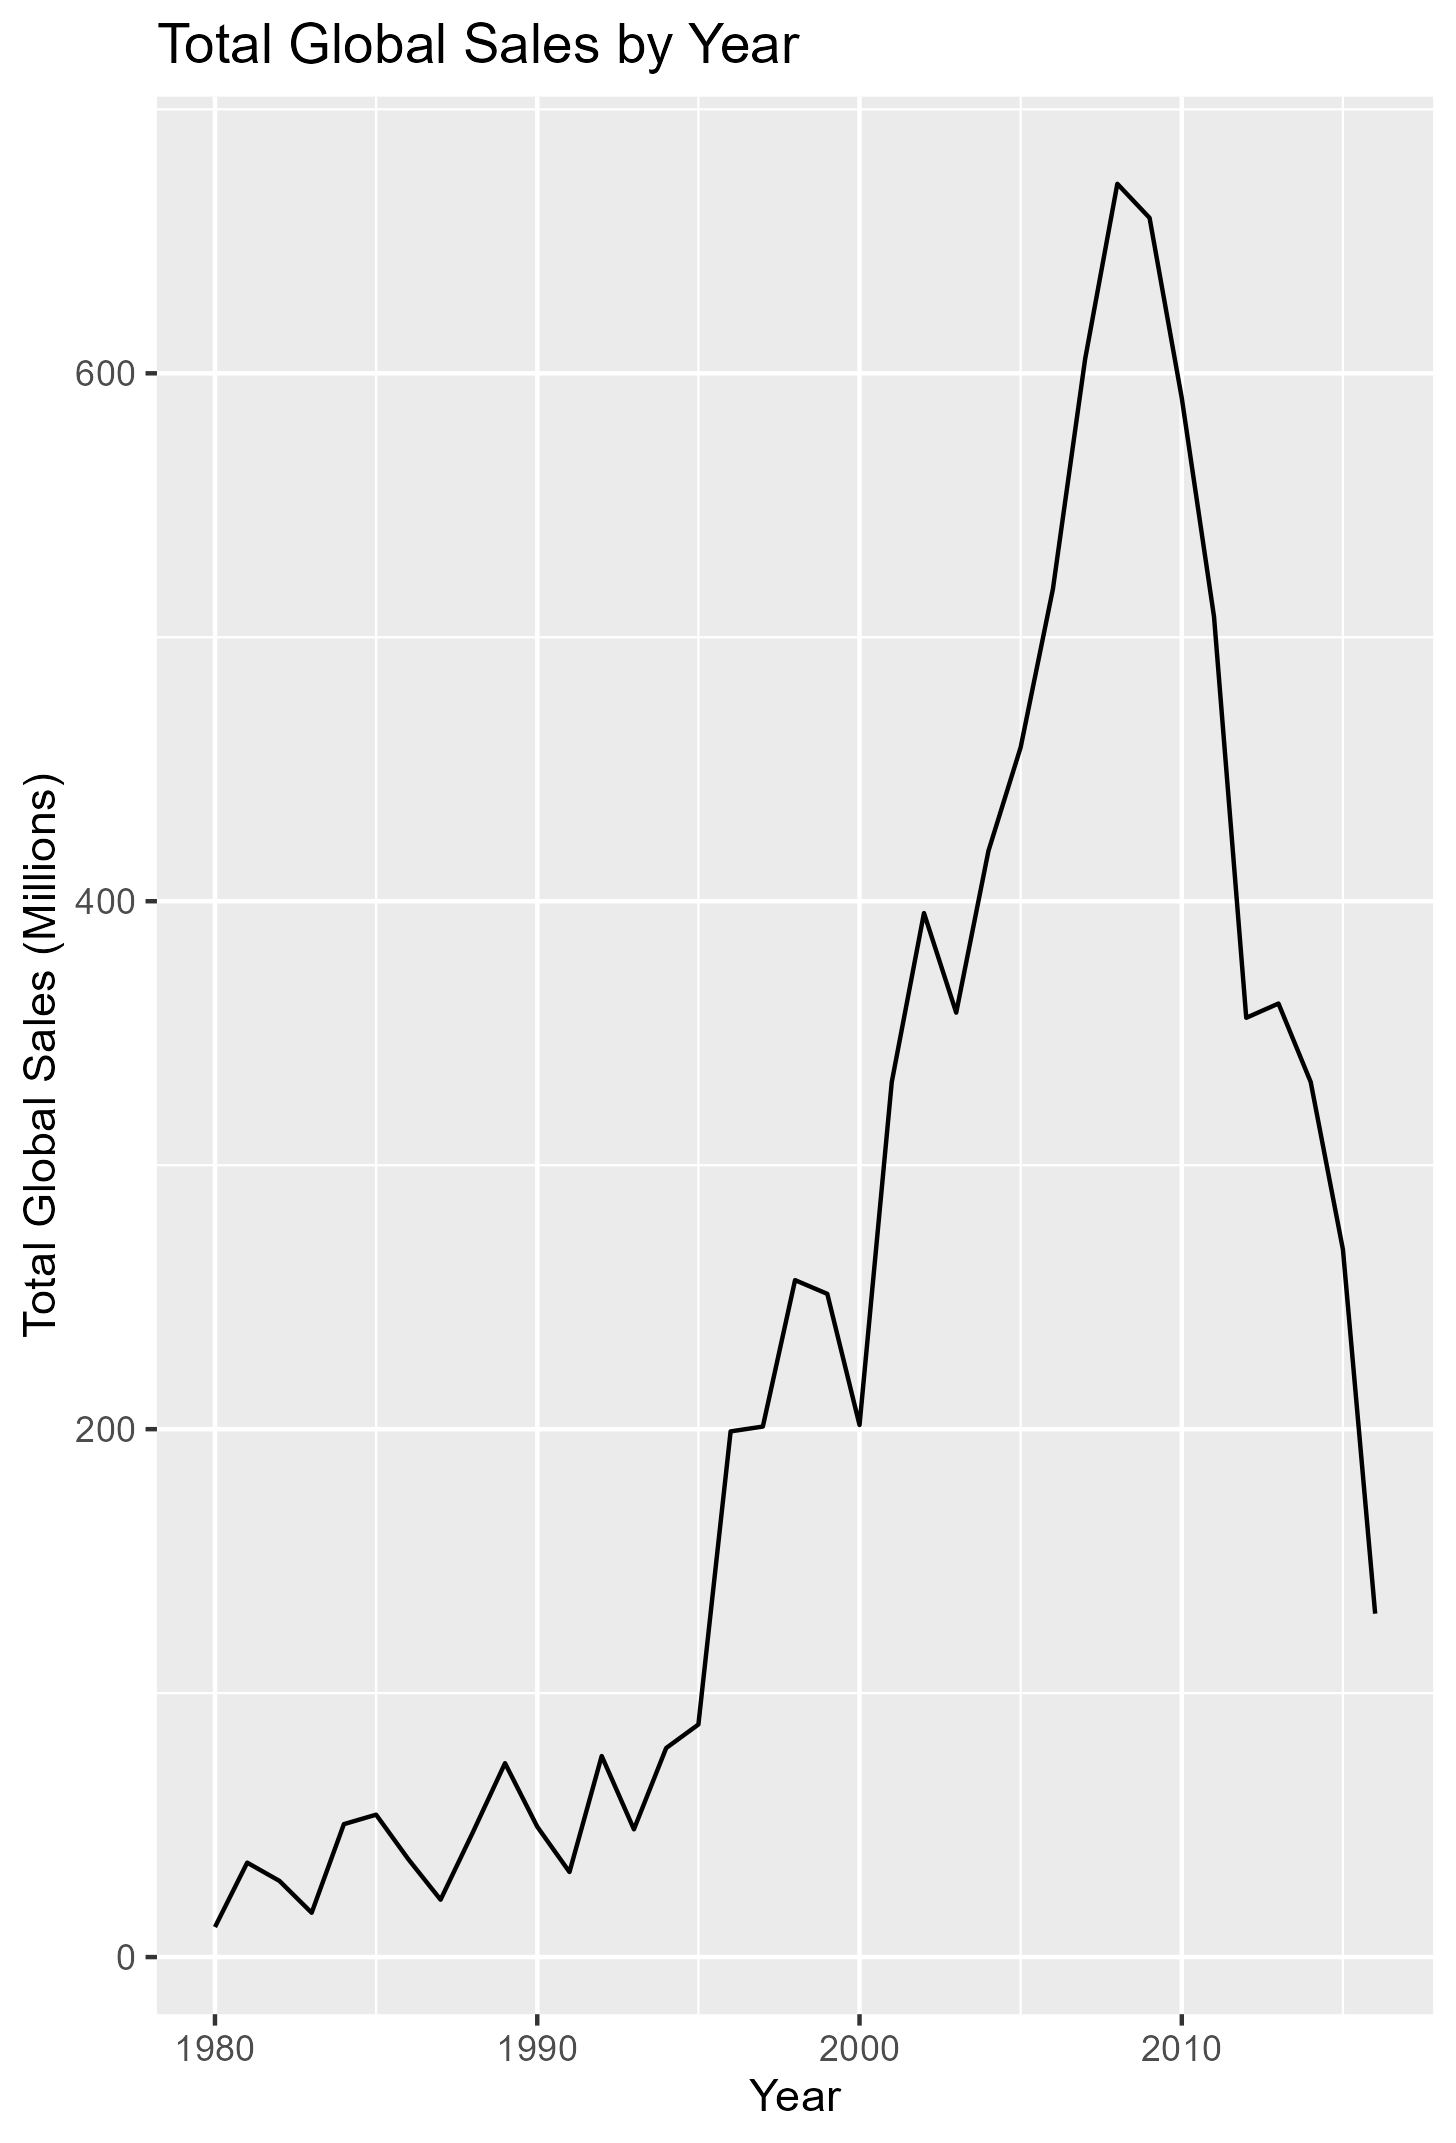
\includegraphics[width=\linewidth]{Figures/total_sales_year.png}
    \caption{Line graph depicting the total number of video games sales per year from 1980-2016}
    \label{fig:fig1}
\end{subfigure}
\begin{subfigure}{0.49\linewidth}
    \centering
    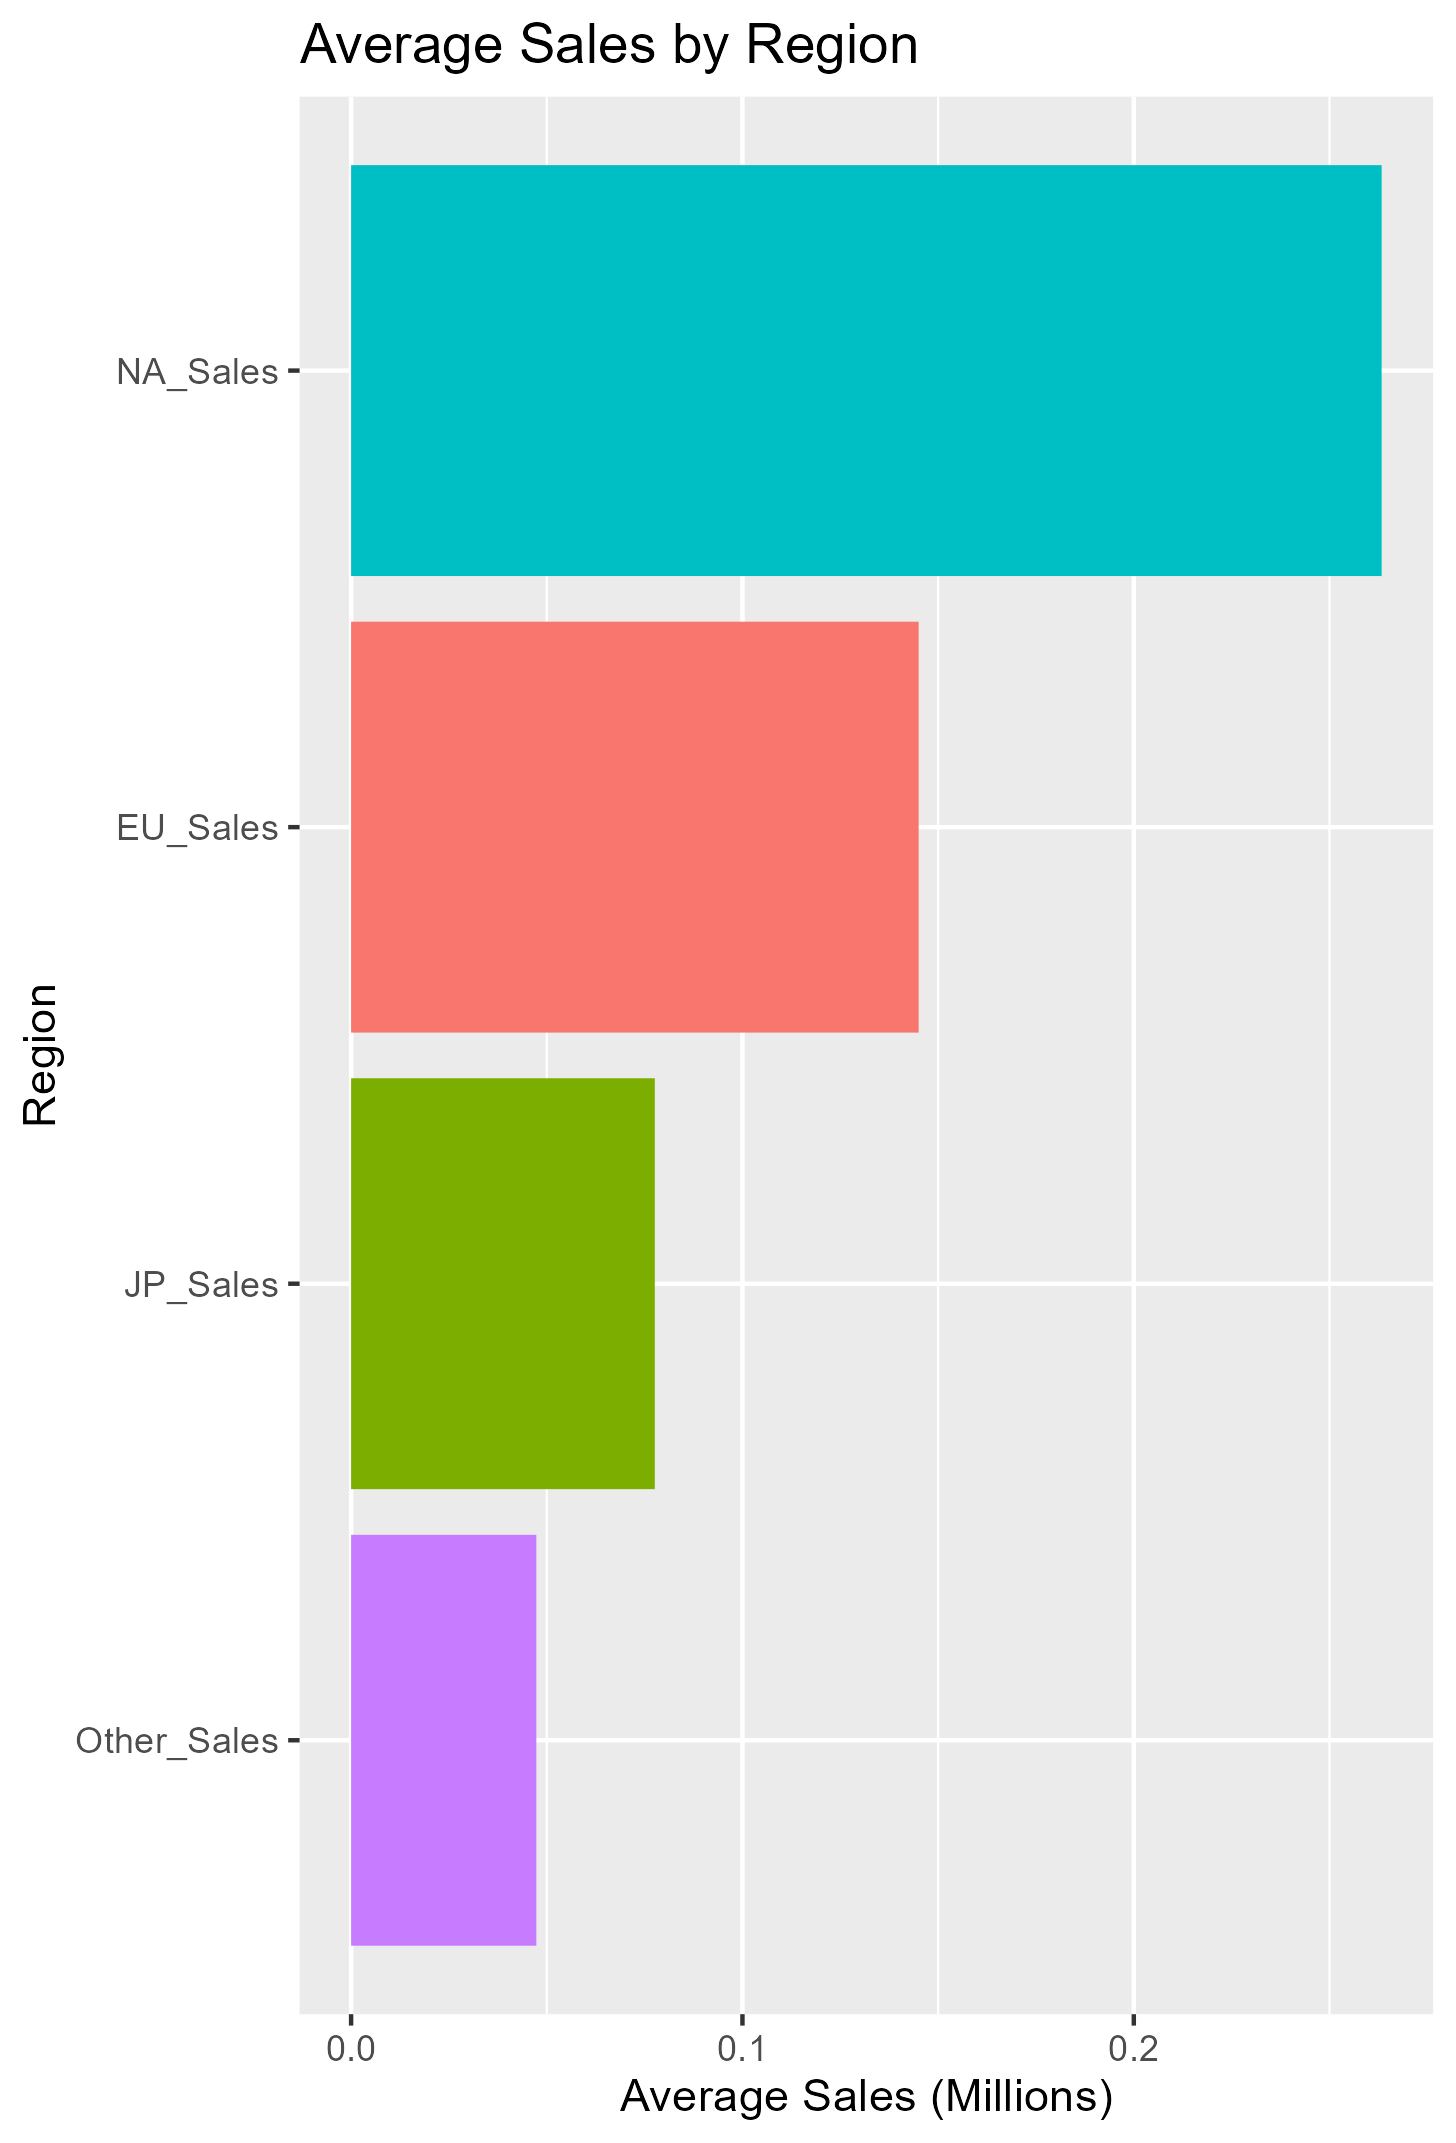
\includegraphics[width=\linewidth]{Figures/avg_sales_region.png}
    \caption{Average Number of Sales by Region (in millions)}
    \label{fig:fig2}
\end{subfigure}
\label{fig:combined1}
\end{figure}

\newpage
\section{Empirical Methods}\label{sec:methods}
Our goal in this study is to explore the influences of review scores on video games on their overall sales. The primary empirical model can be depicted by the following equation: 

\begin{equation}
\label{eq:1}
    Y_{global} = \beta_{0} + \beta_{1}T_{critic} + \beta_{2} X_{user} + \beta_{3} X_{year} + \varepsilon,
\end{equation}
where $Y_{global}$ is a continuous outcome variable for the total number of sales for a particular video game. Our treatment variable $T$ represents whether the game has a critic review or not. This is differentiated as some games have a critic score while others do not. We chose this over the user reviews as within the gaming industry, the critic reviews are more reputable among the community. Sources like the Metacritic is a one of the go-to resources for consumers seeing how well the game performs. In addition, we are including two covariates based on the data set. The $X_{user}$ covariate represents the game's user average user score. While we are prioritizing the treatment of the critic scores, the user scores can still pose an influence on the sales of the game, so we will incorporate that into our model. The other covariate is $X_{year}$, which is the year the game is released. This is because the gaming sector continues to evolve with new technologies as well as cultural trends gaming developers would incorporate in future installments. Both of these can influence the sales of video games. We may expect that games released more recently given the advancements in technology. However, retro-released games may garner higher sales given the culture breakthroughs those games brought during the earlier decades. Thus, there seems to be a trade-off between these factors as whether players prefer newer technologies like graphics or games that have cultural significance. We will utilize three different methods seeing the effect of the critic review scores on the video game sales. First is a linear regression using the model above using robust standard errors. This will produce coefficients and the accompanying p-values to determine the level of significance. To address possible correlations among the covariates, we will a run a another robust regression incorporating the interaction term between user score and release year. This can allow us to see if the treatment effect of the critic score is dependent on these factors. Finally, to ensure consistency with first regression model, we will calculate an estimated average treatment effect difference by splitting the data between games that have and do not have critic review scores. Then, we will calculate the averages in the global sales and take the difference between the two. We would expect a similar average treatment effect with these two methods. 

\section{Research Findings}\label{sec:results}
Now then, let’s discuss our main findings from this analysis. Upon examining our initial 
regression model, we find that as critic score increases, the average global sales of a gaming 
product appears to increase by about .039, or by approximately 400 people in response to a 1 
point increase in critic scores. To the degree that this estimate is valid, we note that with a r value 
of 18.192, this estimation holds at even a 99\% confidence test, also with small standard error of 
.002, this estimate of around 400 people rounds to be quite accurate on average. This appears to 
dismiss the notion that official sources are no longer seen as reputable by the gaming community 
and have little effect on games sales as promoted in other articles. To this end, as our data 
extends from 1980 to 2016, this appears to show that while the credibility of official sources has 
been diminished over time, their overall use as sources of information for a game has largely 
stayed intact and has not yet been completely changed by this issue. Furthermore, as we have 
accounted for year within our analysis, and we have seen that on average games that simply have 
reviews in general appear to fair better than their non reviewed counterparts with a sales boost of 
about .03, this removes any interpretation that these changes occurred due to other factors such 
as popularity. On that note however, there is somewhat of a concerning finding seen in our 
estimated effects of consumer scores, as with a result of -.01 it appears that as consumer scores 
rise the sales of the game decreases by around 100 people. This however, may be due to a 
confounding effect of the rise of gaming popularity over the past few decades. In particular, as 
gaming has become increasingly popular over the past few years, an incredible amount of 
differing people have begun to interact with the gaming industry. Because of this, and the 
subjective nature of game appreciation, there is now going to be higher consumer scores on 
average for all games as a flood of subjective opinions which all appreciate different gaming 
aspects have entered sphere. To this end, as consumer scores in general increase, this means that 
even though some games may not sell well due to low advertising budgets and topics of the like, 
they will still have a high consumer score, which then indirectly conflates high consumer scores 
with low selling games although they are not the cause of these low sales. This is reflected in our 
figure examining user scores and sales, as it can be clearly seen that the majority of scores are 
always high regardless of sales, with very games being rated poorly in consumer scores in 
general. This interpretation of the score may be questioned as one notices that sales have actually 
dropped with year in our figure and regression with a estimate of -.006 which imply lowering 
popularity, however this effect is not notable, as its t-value fails to pass a 90\% confidence 
interval at 1.584. Furthermore, even if it was notable, this drop in sales in later years is likely due 
to the limitations of our data set only covering console releases, as within the 2010’s PC gaming 
began to go on the rise with large amounts of games beginning to be released on Steam which 
shifted the player base around, not due to a drop in gaming’s overall popularity. Thus with this 
critical understanding of the limitations seen within the data, we find that this main interpretation 
of the confounding of consumer scores due to an overall popularity increases in gaming, still 
holds weight. Thus overall, as we evaluate our findings in this data, it appears that critic scores 
still appear to hold weight as sources of information, with even minute shifts within this score 
heavily affecting the overall sales of the game with recent trends in the perception of these scores 
failing to affect their performance. Meanwhile, for consumer scores, it appears that as these 
ratings have largely lost their effect as strong indicators of game quality, as the rise in popularity 
of gaming has lead to an over-saturation of high ranking scores from the public which limits their 
ability to affect sales.


\section{Conclusion}\label{sec:conclusion}
From these findings, we can conclude with three main implications. Firstly, for gaming 
companies the knowledge that critic reviews are so influential to the sales of the game this 
implies that an investment in attaining positive reviews for the game is a fruitful endeavor and 
should be a key component towards the advertising of the game. As we’ve seen that the effect of 
reviews on sales gets diluted when all reviews are positive in consumer reviews, this provides a 
hopeful model that gaming companies have an incentive to ensure reviews are honest in order to 
not dilute this effect. On a similar note, this also implies that businesses have an distinct 
incentive to keep information they present on games truthful, as hordes of positive information 
on a game has been shown through consumer reviews to be ineffective at boosting sales. Lastly, 
our study appears to imply that with the drop in global sales in console gaming over the past 
decade, that business may need to invest in PC portability in order to keep up with other 
companies in the market. In particular, with the affordability of stronger PC’s steadily increasing, 
it appears in this data that this is heavily decreasing sales in the console market, thus in order to 
survive it is likely that companies will need to bridge this platform gap due to the extreme 
advantages PC’ s generally have compared to their console counterparts like customization. 
Overall then, as the gaming industry moves forward we will likely see the continuation of critic 
reviews, unless companies continue to buy these official sources of and the information becomes 
diluted, and with the rise of PC gaming, we may see a decrease in the number of console 
exclusives if companies want to stay around.


\vfill
\pagebreak{}
\begin{spacing}{1.0}
\addcontentsline{toc}{section}{References}
\bibliographystyle{plain}
\bibliography{references}
\end{spacing}

\vfill
\pagebreak{}
\clearpage

\section*{Figures and Tables}\label{sec:figTables}
\addcontentsline{toc}{section}{Figures and Tables}

%========================================
% FIGURES AND TABLES 
%========================================

%----------------------------------------
% Table 1
%----------------------------------------

\begin{table}[ht]
\centering
\caption{Summary Statistics of Video Game Sales 1980-2016}
\label{tab:descriptive-vg}
\begin{tabularx}{\textwidth}{X *{9}{r}} % Use tabularx to adjust column widths and 'r' to right-align numerical columns
\toprule
& \begin{sideways}Release Year\end{sideways} & \begin{sideways}NA\_Sales\end{sideways} & \begin{sideways}EU\_Sales\end{sideways} & \begin{sideways}JP\_Sales\end{sideways} & \begin{sideways}Other\_Sales\end{sideways} & \begin{sideways}Global\_Sales\end{sideways} & \begin{sideways}Critic\_Score\end{sideways} & \begin{sideways}Critic\_Count\end{sideways} & \begin{sideways}User\_Score\end{sideways} \\ 
\midrule
Min. & 1980 & 0.0000 & 0.0000 & 0.00000 & 0.00000 & 0.0100 & 13.00 & 3.00 & 0.00 \\ 
1st Qu. & 2003 & 0.0000 & 0.0000 & 0.00000 & 0.00000 & 0.0600 & 60.00 & 12.00 & 64.00 \\ 
Median & 2007 & 0.0800 & 0.0200 & 0.00000 & 0.01000 & 0.1700 & 71.00 & 22.00 & 75.00 \\ 
Mean & 2006 & 0.2641 & 0.1459 & 0.07848 & 0.04759 & 0.5364 & 68.99 & 26.44 & 71.26 \\ 
3rd Qu. & 2010 & 0.2400 & 0.1100 & 0.04000 & 0.03000 & 0.4700 & 79.00 & 36.00 & 82.00 \\ 
Max. & 2016 & 41.3600 & 28.9600 & 10.22000 & 10.57000 & 82.5300 & 98.00 & 113.00 & 97.00 \\ 
NA's & & & & & & & 8463 & 8463 & 8983 \\ 
\bottomrule
\end{tabularx}
\end{table}

%----------------------------------------
% Table 2
%----------------------------------------

\begin{table}[ht]
\centering
\caption{Linear Regression Results }
\label{tab:regression_results}
\begin{tabular}{lcccccc}
\toprule
\textbf{Variable} & \textbf{Estimate} & \textbf{Std. Error} & \textbf{t value} & \textbf{Pr($>|t|$)} & \textbf{CI Lower} & \textbf{CI Upper} \\
\midrule
Intercept & 11.963 & 8.348 & 1.433 & 0.152 & -4.401 & 28.327 \\
Critic\_Score & 0.040 & 0.002 & 18.192 & $< 0.001$ & 0.036 & 0.044 \\
User\_Score & -0.011 & 0.002 & -6.170 & $< 0.001$ & -0.014 & -0.007 \\
Year\_of\_Release & -0.007 & 0.004 & -1.584 & 0.113 & -0.015 & 0.002 \\
\bottomrule
\end{tabular}
\end{table}

%----------------------------------------
% Table 3
%----------------------------------------

\begin{table}[ht]
\centering
\caption{Regression Results Using Interaction Terms}
\label{tab:regression_results_2}
\begin{tabular}{lcccccc}
\toprule
\textbf{Variable} & \textbf{Estimate} & \textbf{Std. Error} & \textbf{t value} & \textbf{Pr($>|t|$)} & \textbf{CI Lower} & \textbf{CI Upper} \\
\midrule
Intercept & -62.53 & 38.37 & -1.630 & 0.103 & -137.7 & 12.68 \\
Critic\_Score & 0.040 & 0.002 & 18.312 & $< 0.001$ & 0.035 & 0.044 \\
User\_Score & 1.016 & 0.571 & 1.779 & 0.075 & -0.104 & 2.135 \\
Year\_of\_Release & 0.031 & 0.019 & 1.596 & 0.111 & -0.007 & 0.068 \\
User\_Score:Year\_of\_Release & -0.00051 & 0.00028 & -1.795 & 0.073 & -0.00107 & 0.00005 \\
\bottomrule
\end{tabular}
\end{table}


%----------------------------------------
% Figures
%----------------------------------------
\begin{figure}[ht]
\centering
\begin{subfigure}{0.49\linewidth}
    \centering
    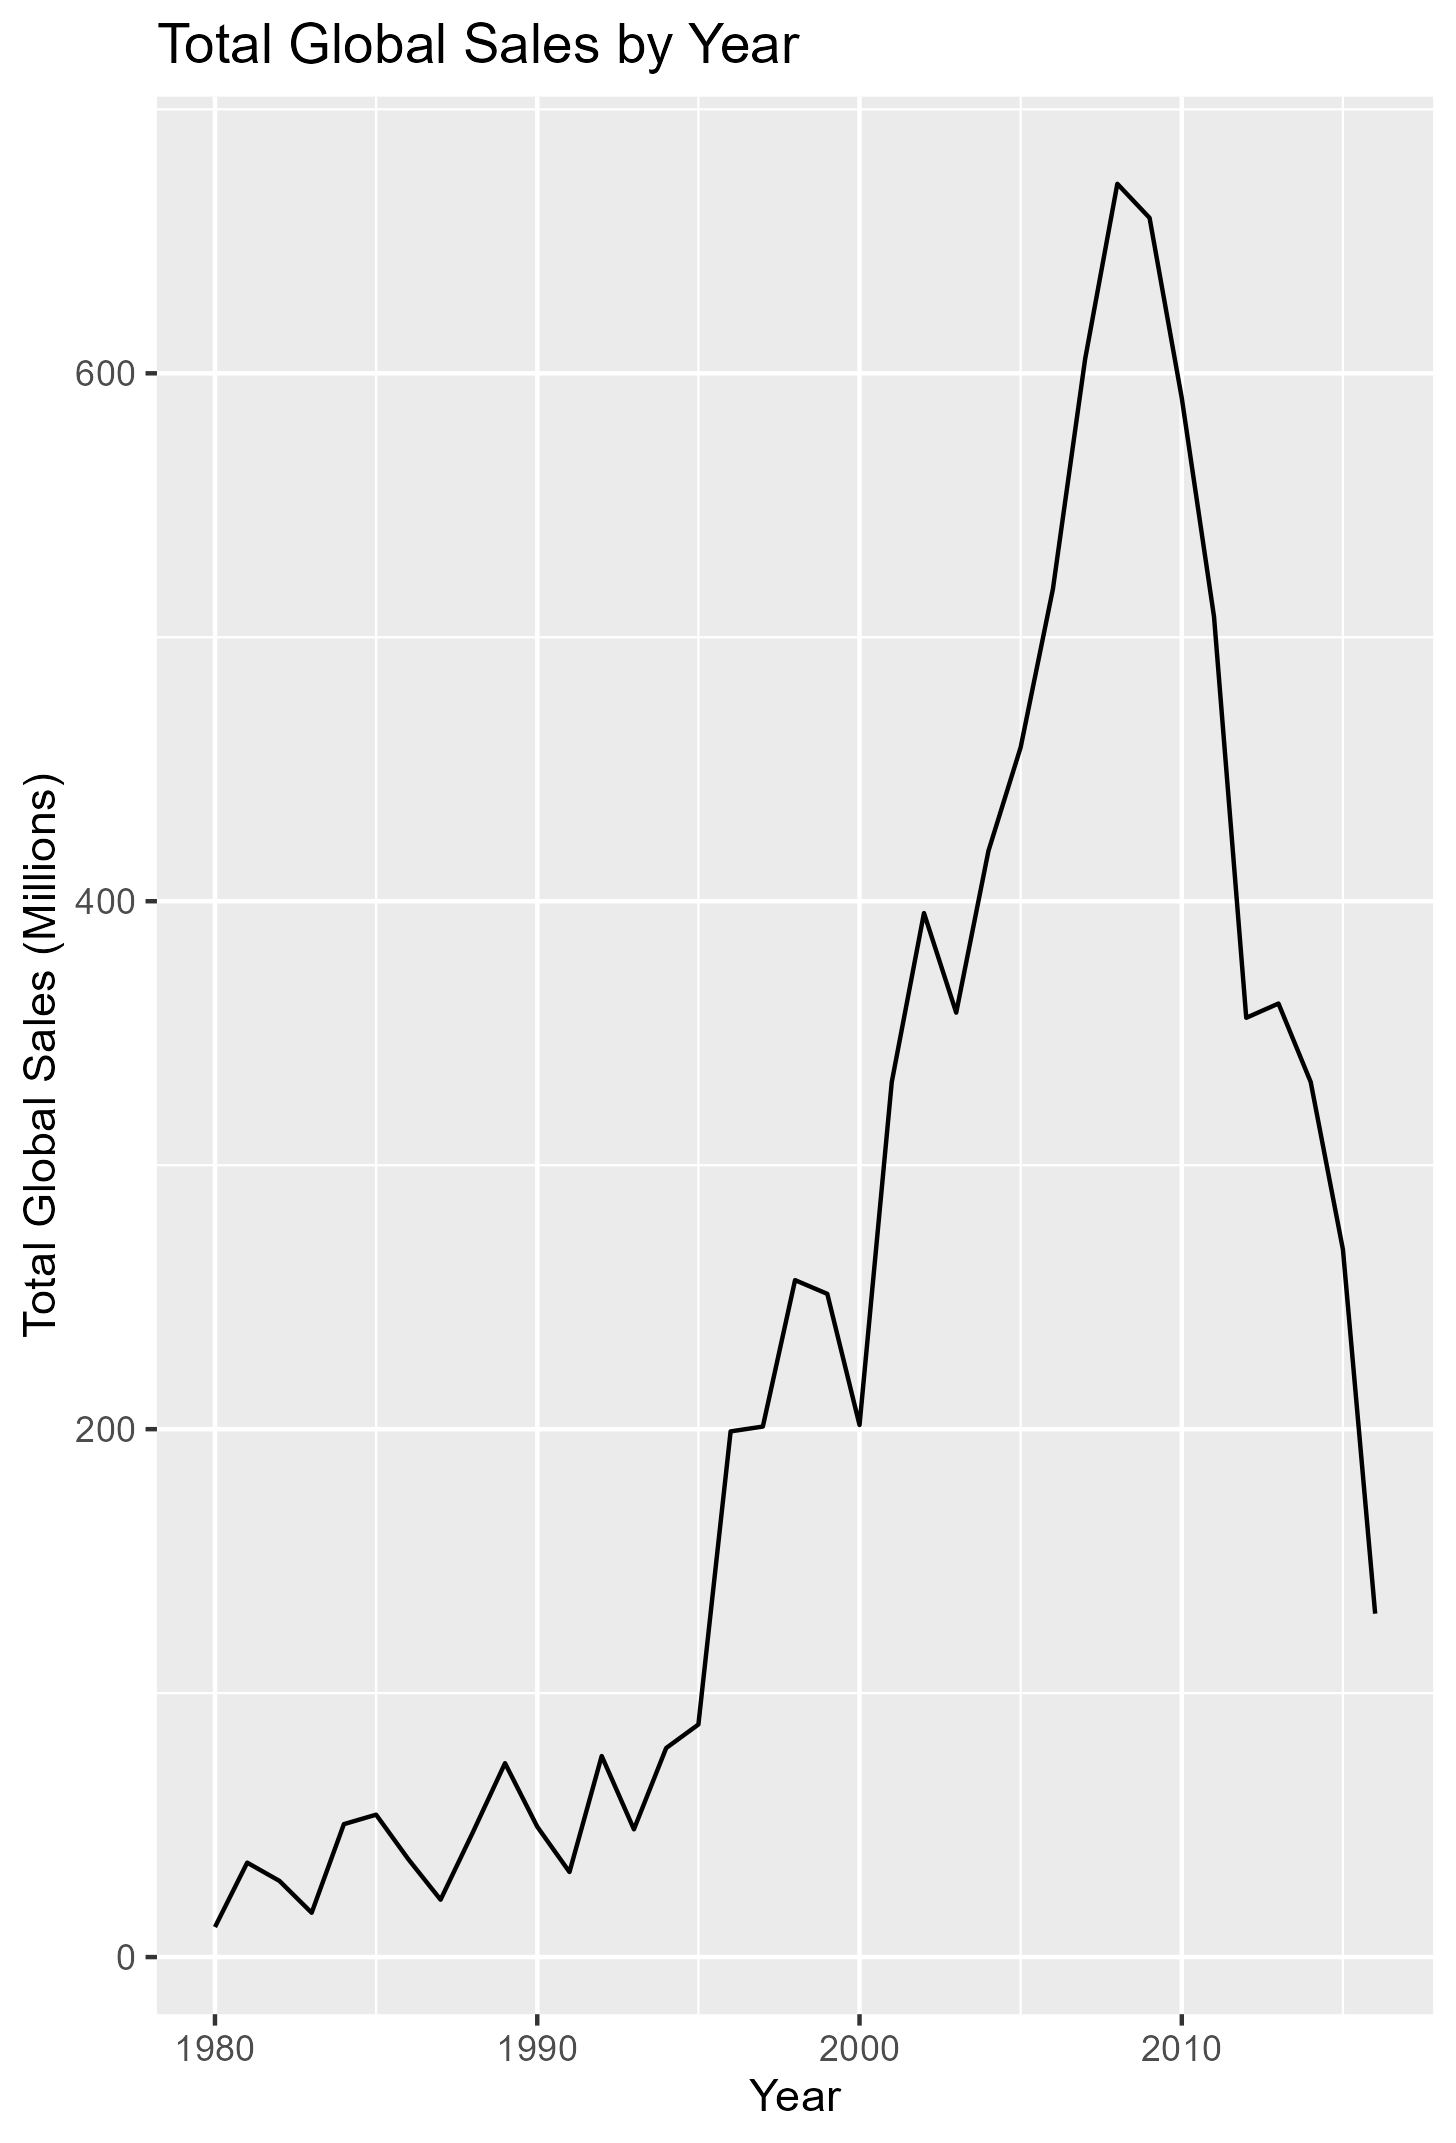
\includegraphics[width=\linewidth]{Figures/total_sales_year.png}
    \caption{Line graph depicting the total number of video games sales per year from 1980-2016}
    \label{fig:fig1}
\end{subfigure}
\begin{subfigure}{0.49\linewidth}
    \centering
    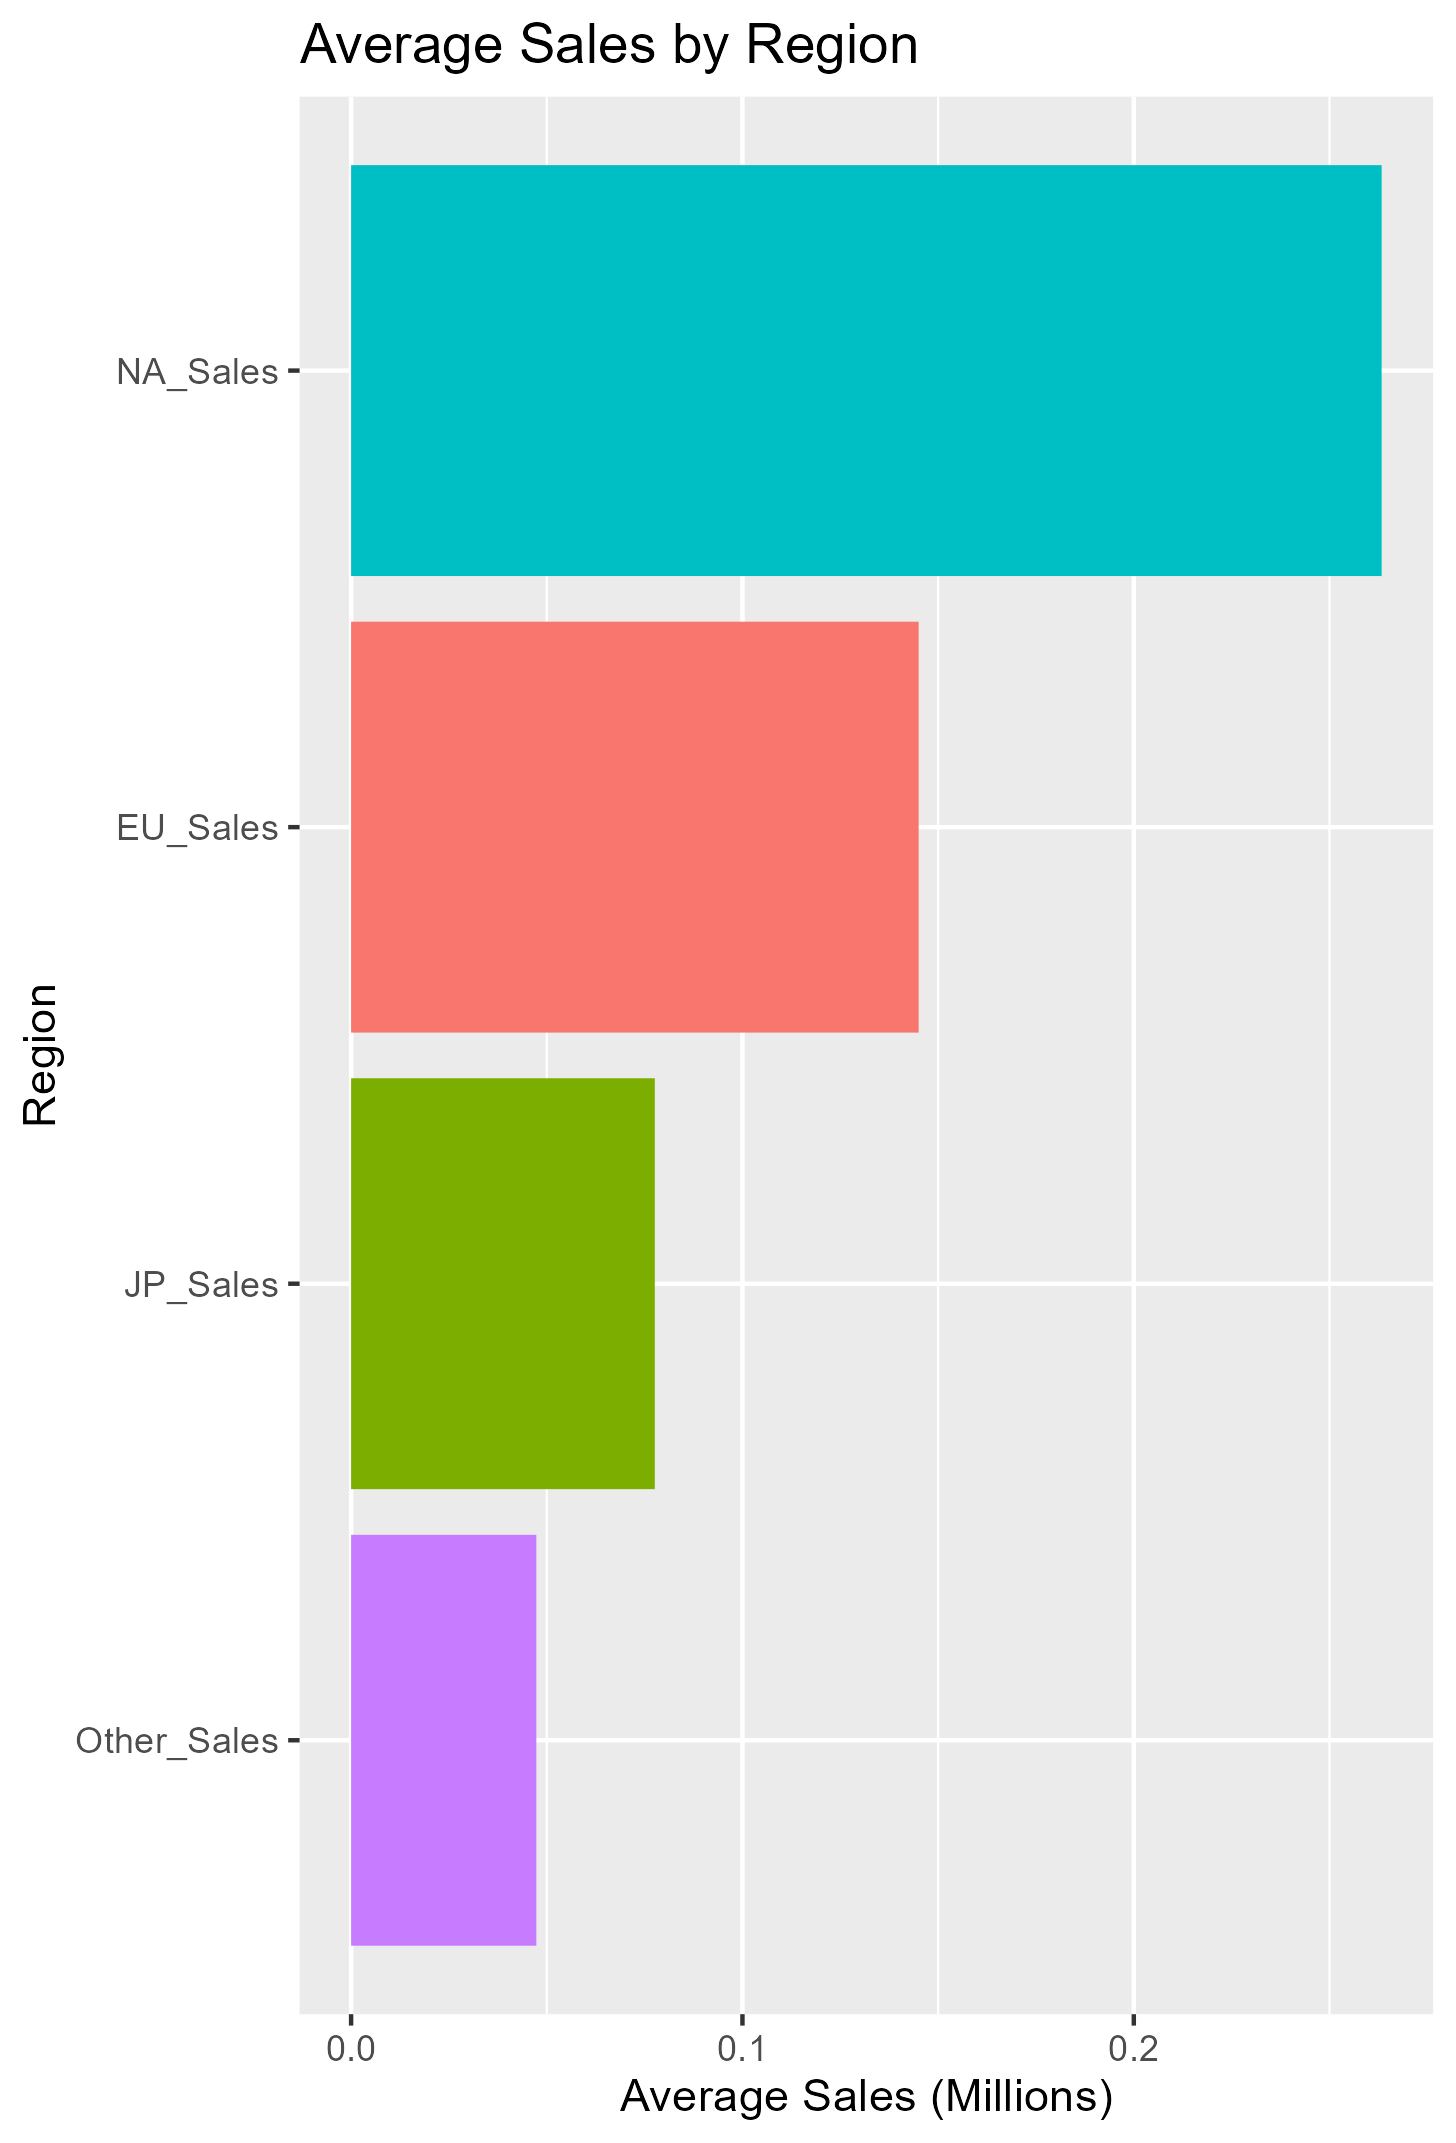
\includegraphics[width=\linewidth]{Figures/avg_sales_region.png}
    \caption{Average Number of Sales by Region (in millions)}
    \label{fig:fig2}
\end{subfigure}
\label{fig:combined1}
\end{figure}

\begin{figure}[ht]
\centering
\begin{subfigure}{0.49\linewidth}
    \centering
    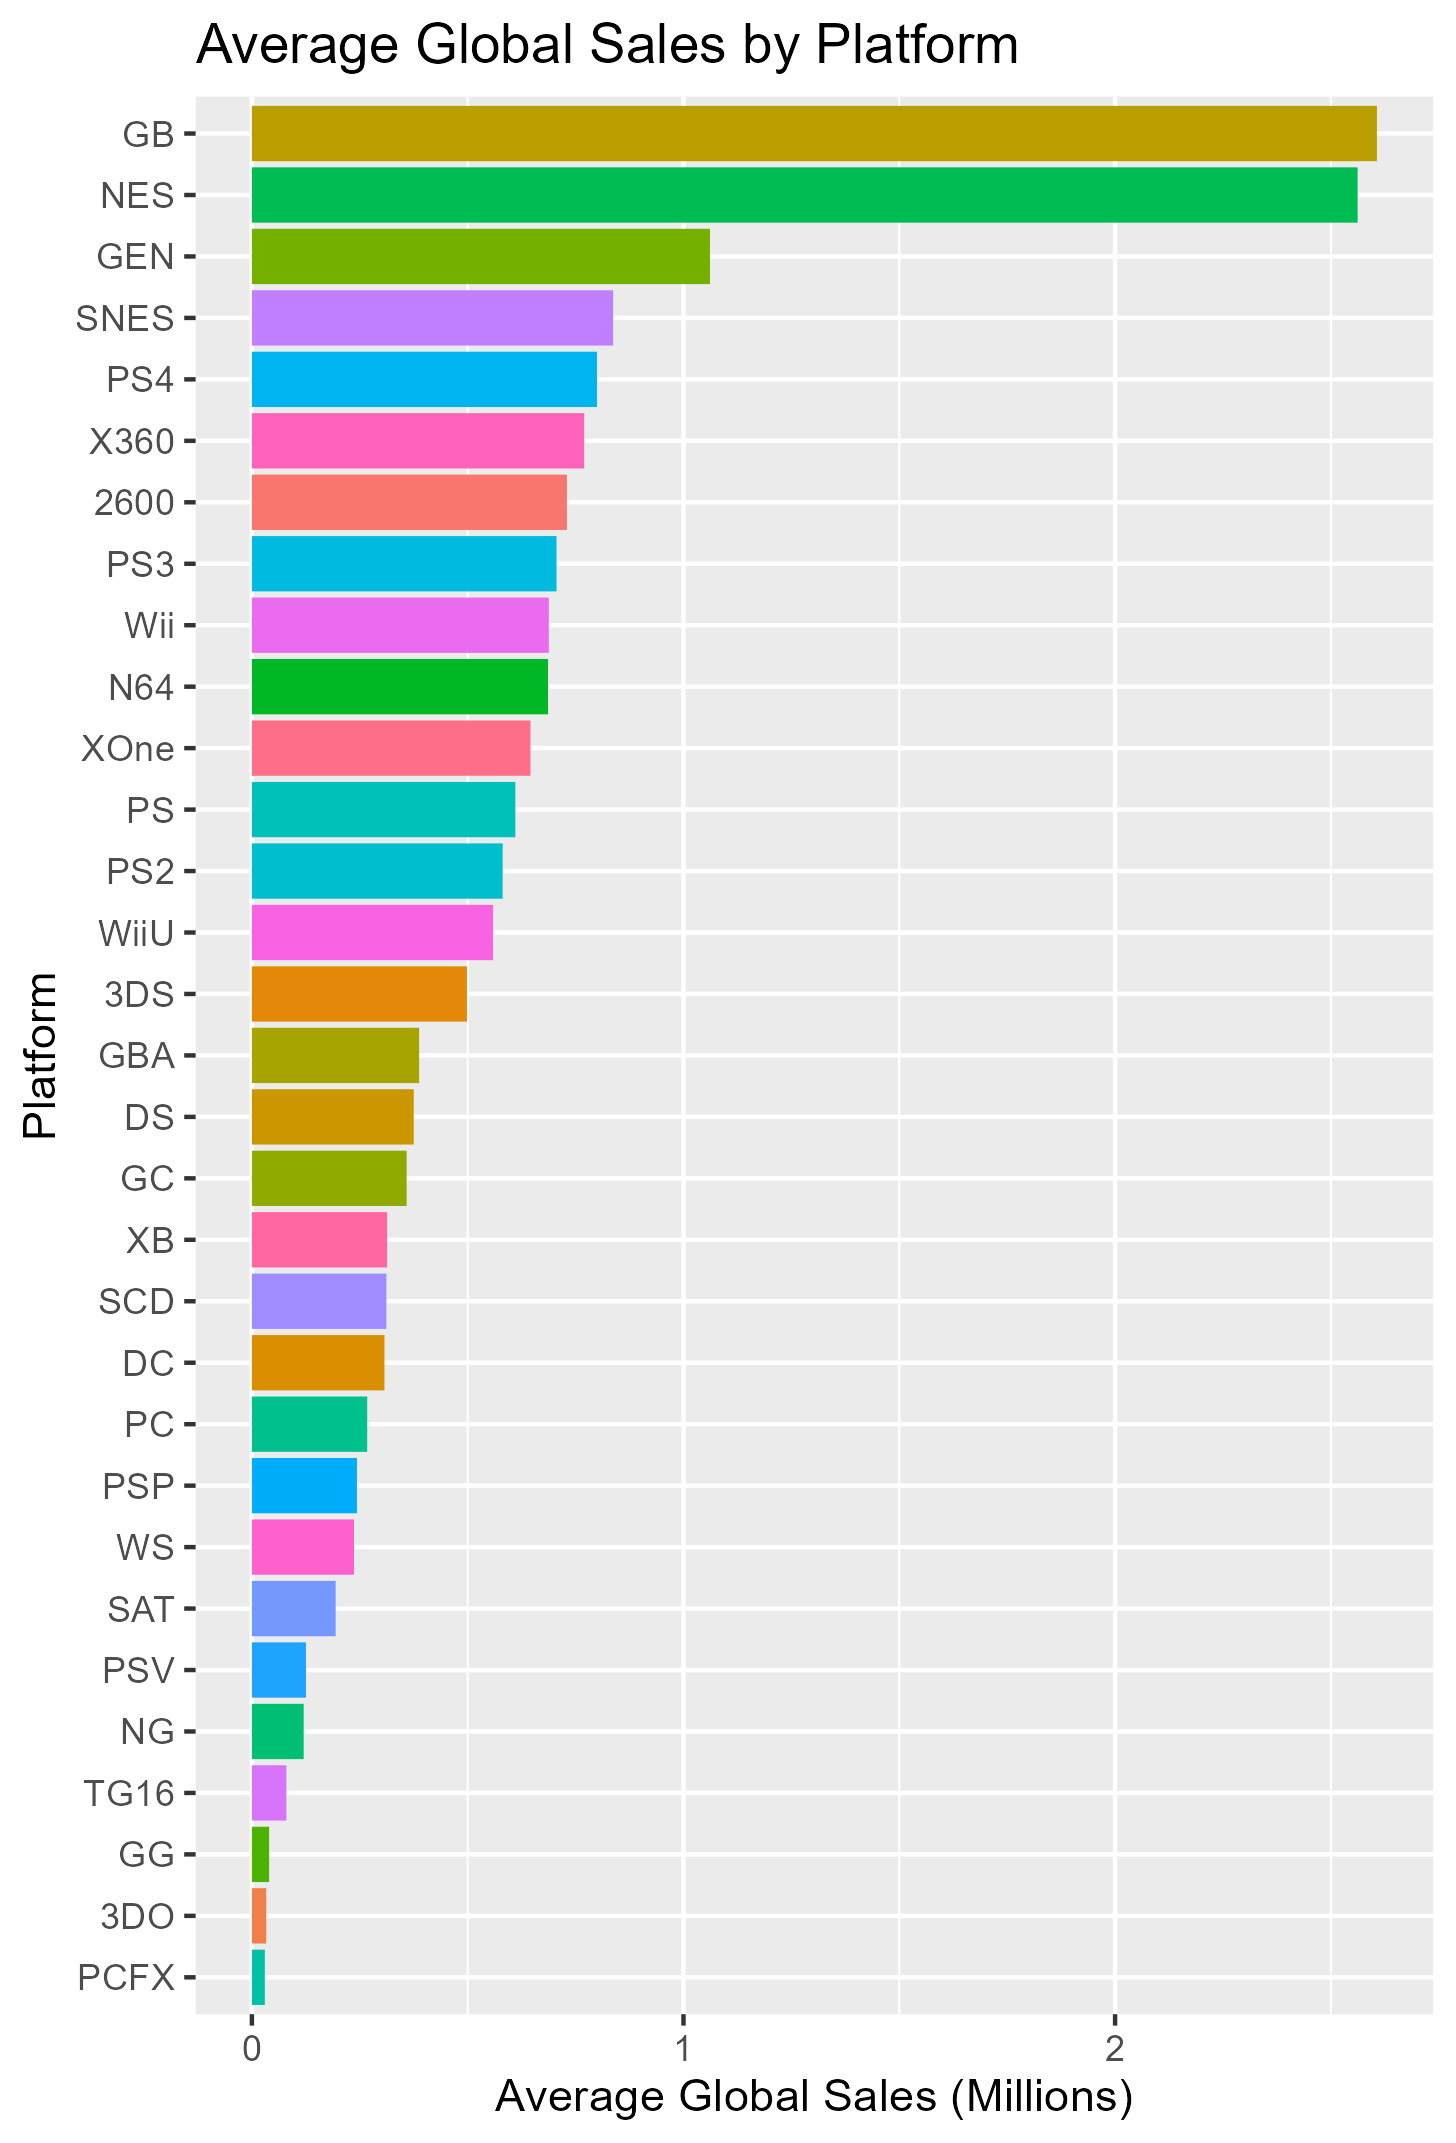
\includegraphics[width=\linewidth]{Figures/avg_sales_platform.png}
    \caption{Average Number of Sales per Gaming Platform}
    \label{fig:fig3}
\end{subfigure}
\begin{subfigure}{0.49\linewidth}
    \centering
    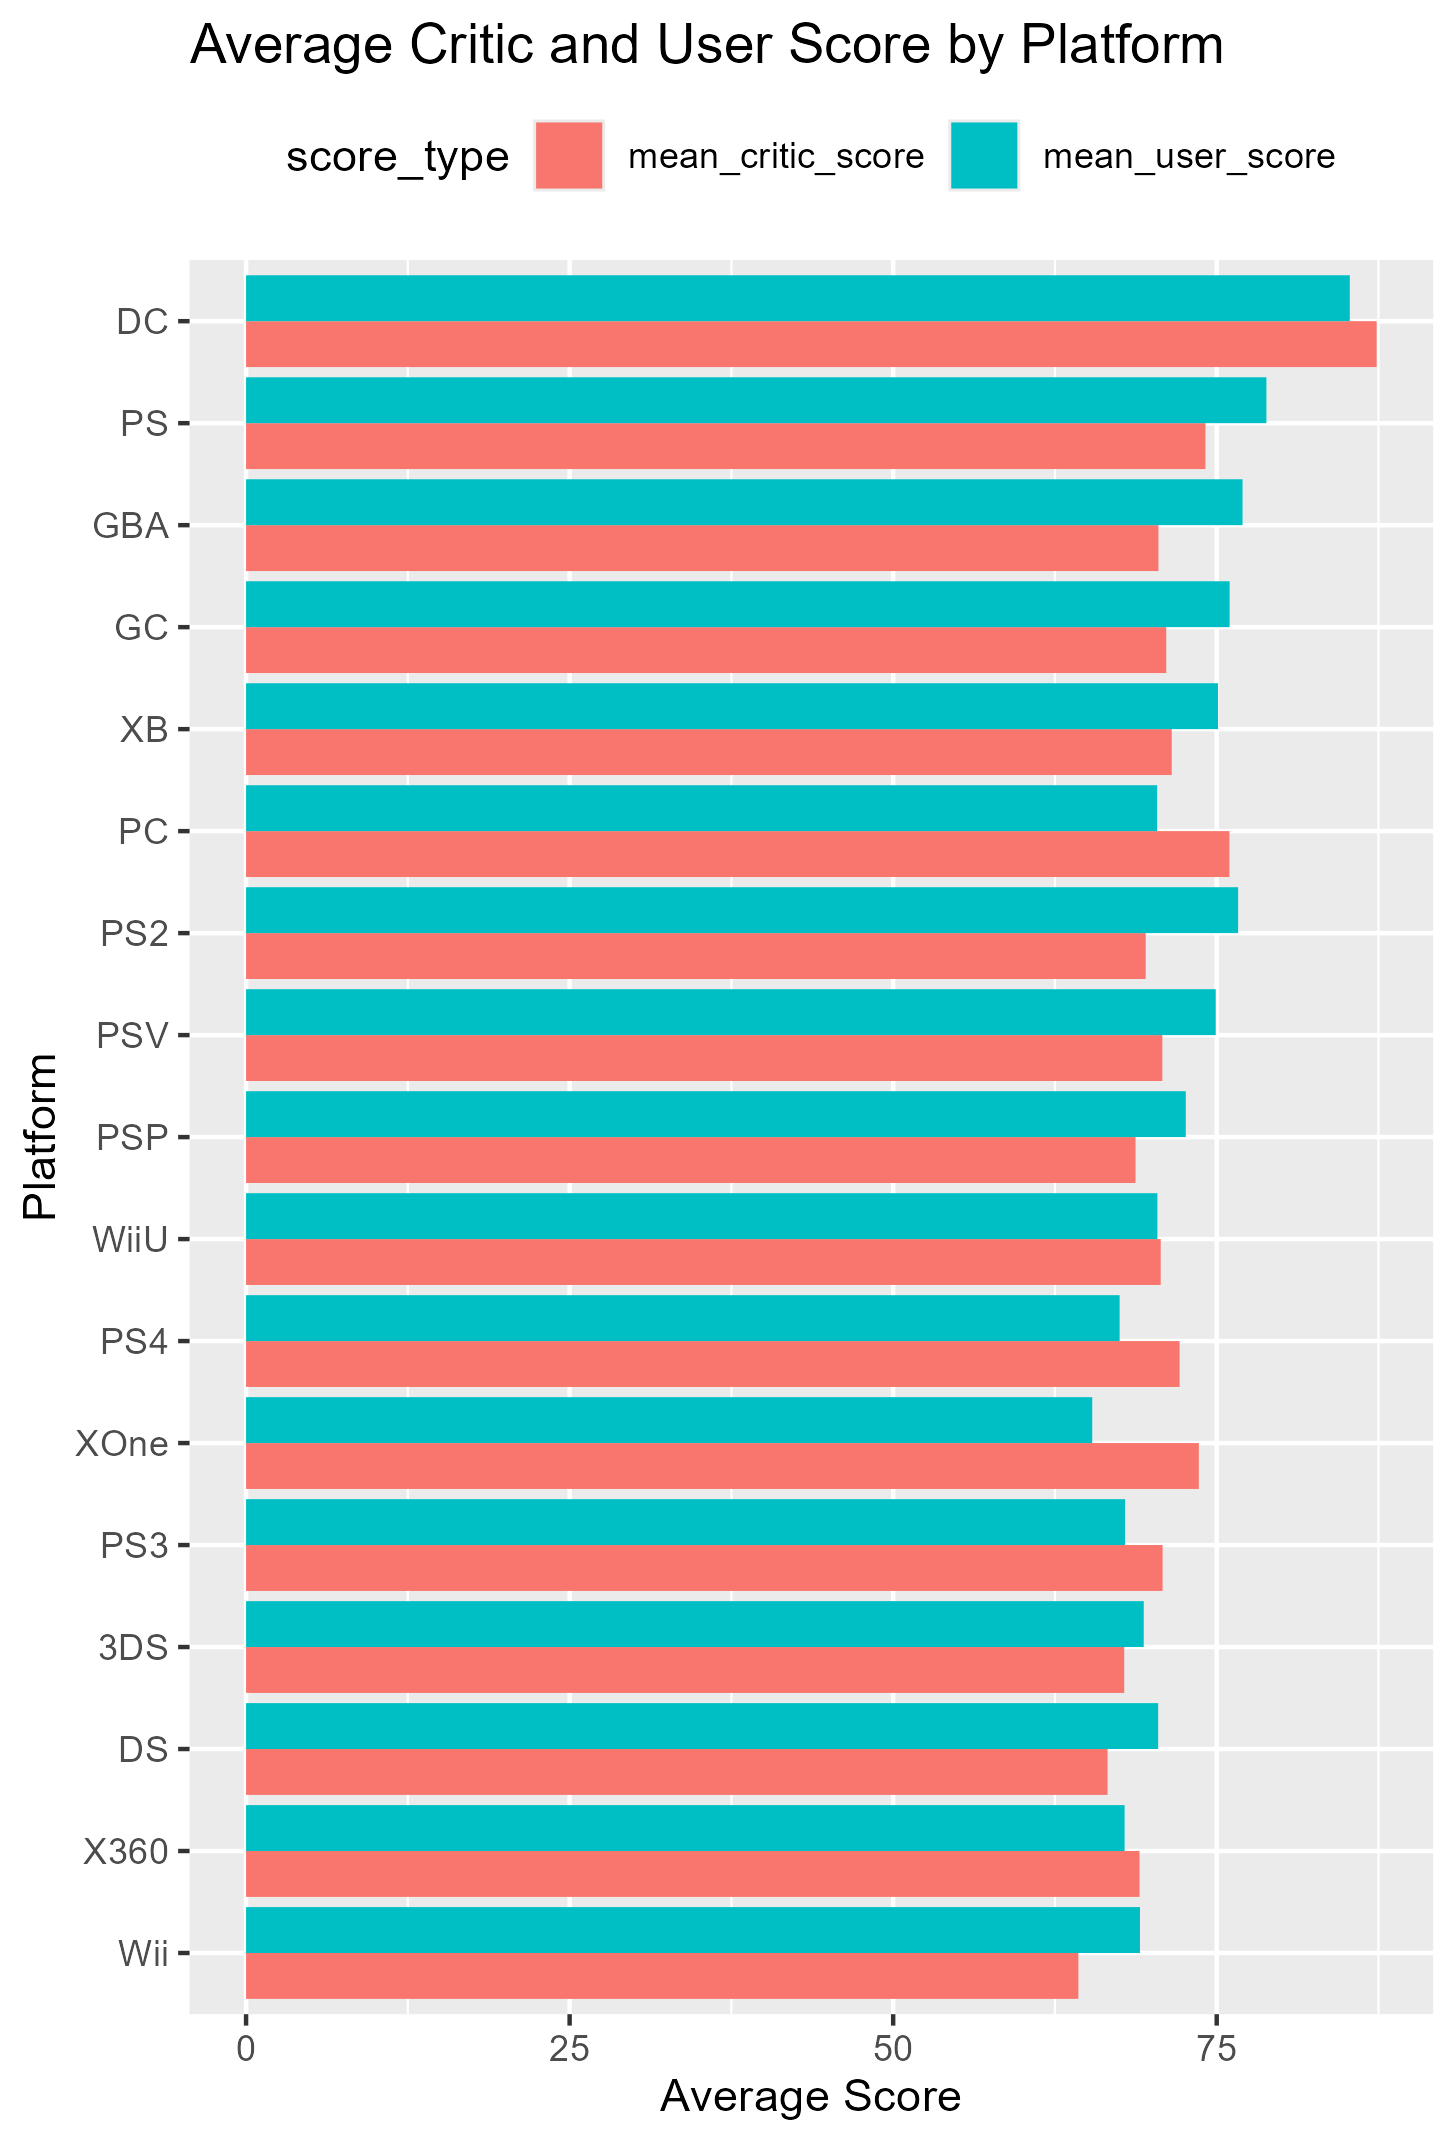
\includegraphics[width=\linewidth]{Figures/avg_scores_platform.png}
    \caption{Average Critic and User Score by Platform}
    \label{fig:fig4}
\end{subfigure}
\label{fig:combined2}
\end{figure}

\begin{figure}[ht]
\centering
\begin{subfigure}{0.49\linewidth}
    \centering
    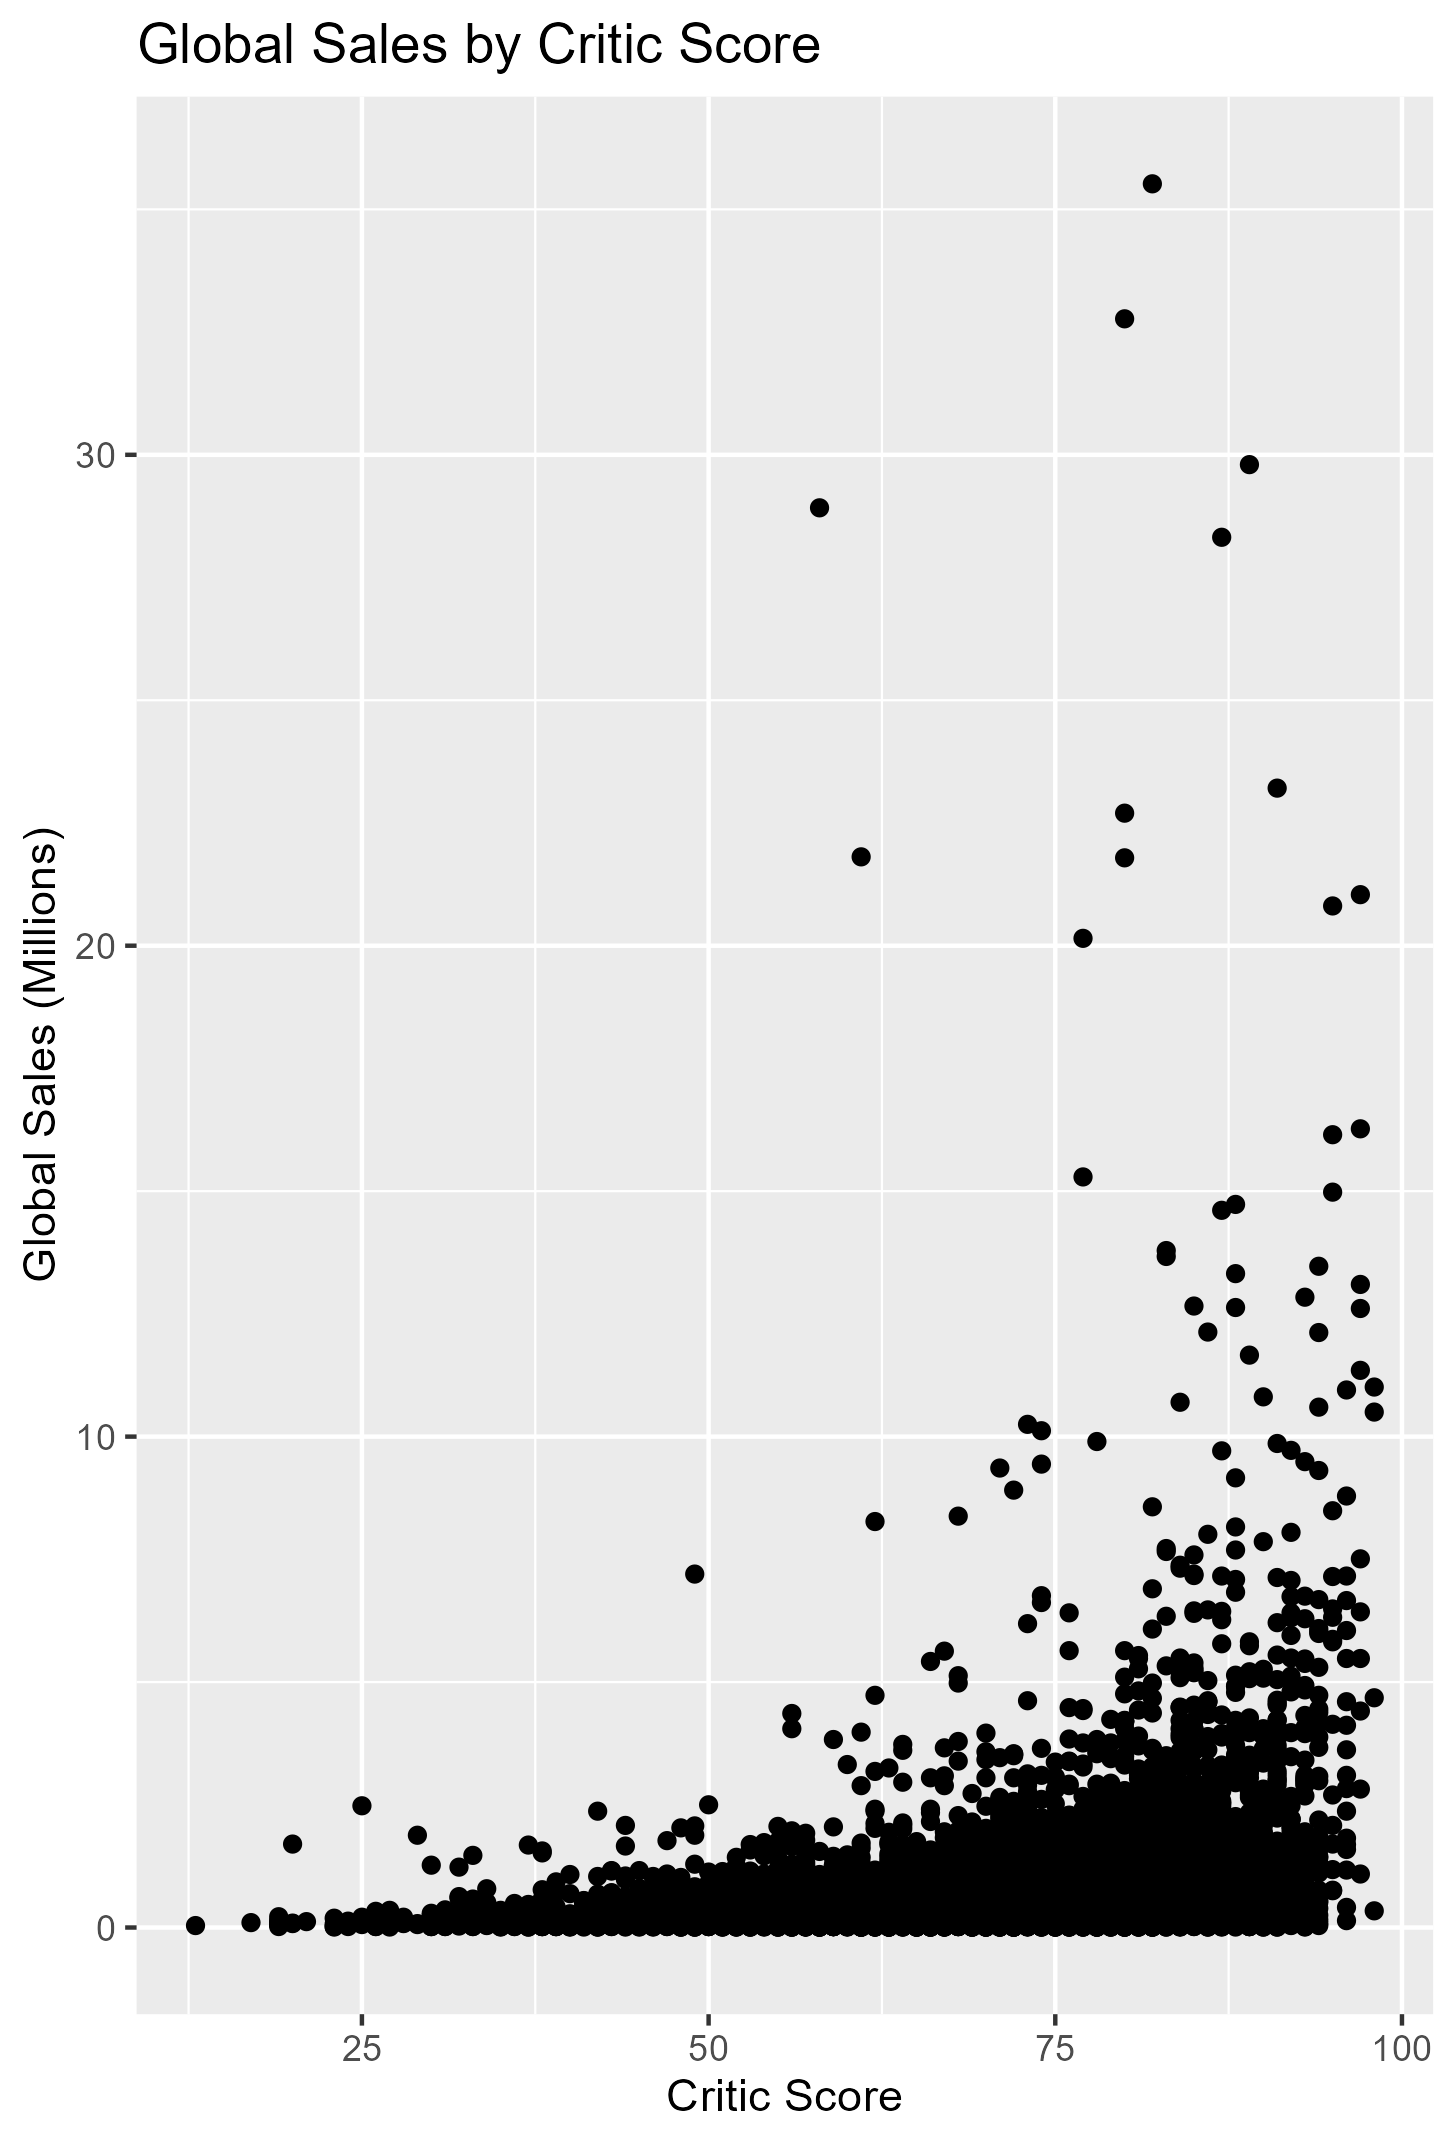
\includegraphics[width=\linewidth]{Figures/sales_critic_score.png}
    \caption{Global Sales Based on Critic Score}
    \label{fig:fig5}
\end{subfigure}
\begin{subfigure}{0.49\linewidth}
    \centering
    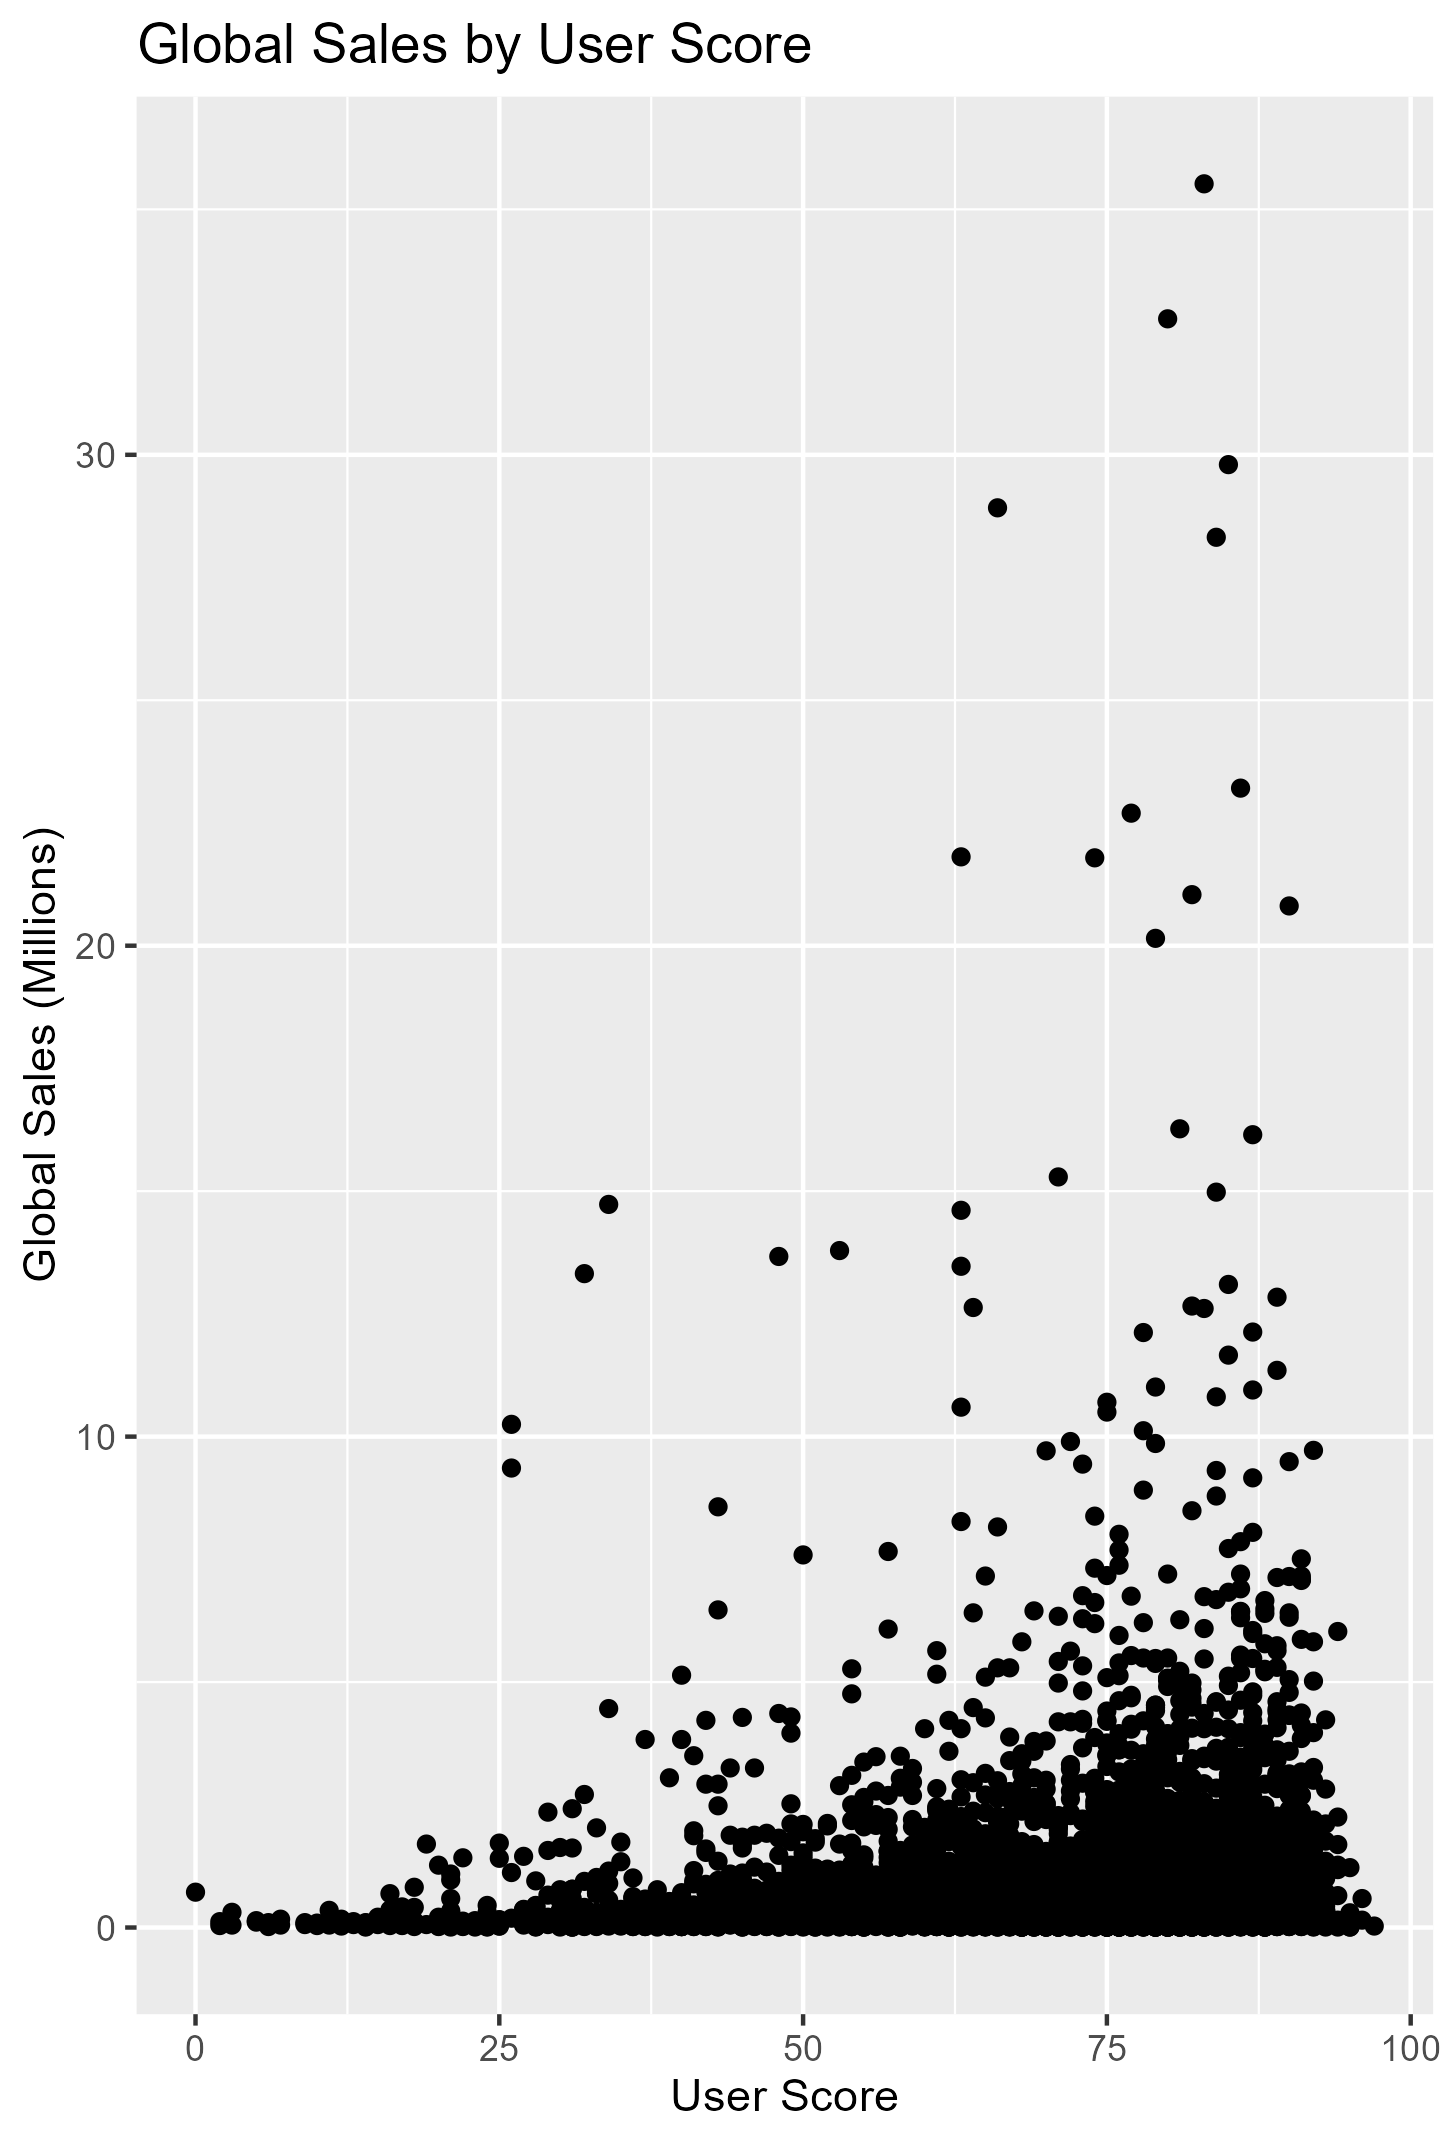
\includegraphics[width=\linewidth]{Figures/sales_user_score.png}
    \caption{Global Sales Based on User Score}
    \label{fig:fig6}
\end{subfigure}
\label{fig:combined3}
\end{figure}

\end{document}
